\begin{mainquestion}{cstransfer}{Biasing, Clipping, and Signal Swing}

\questionpoints
Consider a common source (CS) amplifier shown in figure (a) below. The key parameters are $R_D = 8.5 \text{ k}\Omega$, $V_{DD} = 10 \text{ V}$, $k_n = k_n'\frac{W}{L} = 5 \text{ mA/V}^2$, and $V_t = 1 \text{ V}$. Assume $\lambda = 0$ for parts (a)-(d).

\begin{center}
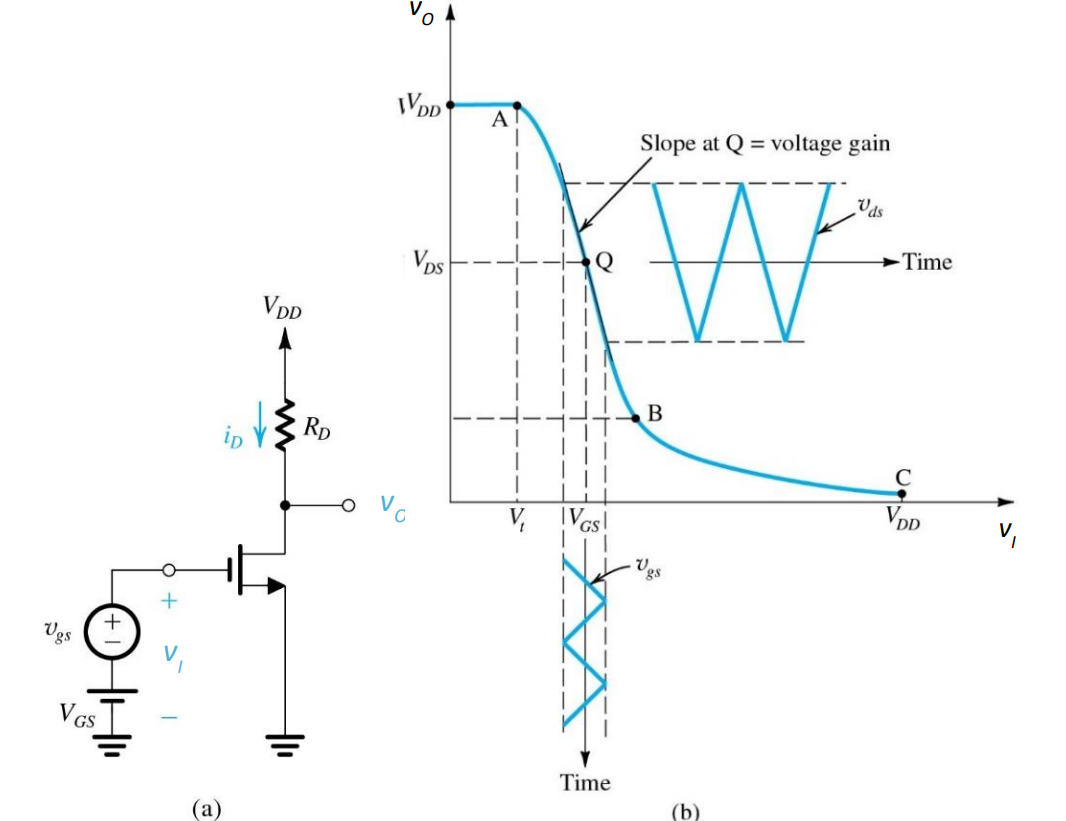
\includegraphics[width=0.8\linewidth]{screenshot_2026_02_23_190651.png}
\end{center}

% =========================================================
\begin{partquestion}{findpointsab}
{Find the coordinates (i.e., $V_I$ and $V_O$) of points A and B on the sketch in figure (b) above. Assume point A marks the transition from the cut-off region to the saturation region, and point B marks the transition from the saturation region to the triode region.}

\begin{answer}
        Point A on the sketch corresponds to the moment when the transistor transitions from cut-off to saturation. This occurs when $v_I = v_{GS} = V_t = 1 \text{ V}$. At this point, current is just beginning to flow so $v_{DS} = v_O = V_{DD}$. So, point A is (1 V, 10 V).

        Point B corresponds to the moment where the transistor goes from saturation to triode. In this case, $v_{DS} = v_{GS} - V_t$ so $v_O = v_I - V_t = v_I - 1 \text{ V}$. Because at point B we are at the boundary of two regions, either formula for $I_D$ should work (also because $\lambda=0$, which ensures continuity between regions with our standard formulas for $I_D$). Choosing that of saturation gives:
        \[I_D = \frac{V_{DD}-v_O}{R_D} = \frac{1}{2}k_n(v_{GS}-V_t)^2\]
        This leads to the quadratic:
        \[\frac{10-v_O}{8.5} = \frac{1}{2}(5)(v_I-1)^2 = \frac{1}{2}(5)v_O^2\]
        \[2.5v_O^2 + 0.1176v_O - 1.1765 = 0\]
        which has solutions $v_O \approx -0.710 \text{ V}$ and $v_O \approx 0.663 \text{ V}$. Only the positive root is a valid solution. From here, $v_I = v_O + 1 \approx 1.663 \text{ V}$, so point B is (1.663 V, 0.663 V).
\end{answer}

\end{partquestion}

% =========================================================
\begin{partquestion}{biaspoint}
{If the amplifier is biased to operate with an overdrive voltage $V_{OV} = V_{GS} - V_t = 0.4 \text{ V}$, what is the output voltage ($V_O$) and input voltage ($V_I$) at that bias point (which we call Q)? What is the DC operating current ($I_D$) at the bias point Q?}

\begin{answer}
        First, we find the required gate-to-source voltage (which is the DC input voltage, $V_I$):
        \[V_I = V_{GS} = V_{OV} + V_t = 0.4 + 1.0 = 1.4 \text{ V}\]
        
        Using the saturation region current equation, we can find the DC operating current $I_D$:
        \[I_D = \frac{1}{2}k_n V_{OV}^2 = \frac{1}{2}(5)(0.4)^2 = 0.4 \text{ mA}\]
        
        Now, we can find the output voltage $V_O$ by calculating the voltage drop across the drain resistor $R_D$:
        \[V_O = V_{DD} - I_D R_D = 10 - (0.4)(8.5) = 6.6 \text{ V}\]
        
        Therefore, the DC operating current is $I_D = 0.4 \text{ mA}$ and the output voltage is $V_O = 6.6 \text{ V}$ (meaning the bias point Q is located at $V_I = 1.4 \text{ V}$, $V_O = 6.6 \text{ V}$).
\end{answer}

\pagebreak
\end{partquestion}

% =========================================================
\begin{partquestion}{maxamplitude}
{At the bias point Q, what is the maximum allowable input signal swing (amplitude) that keeps the transistor in saturation? What is the resulting peak-to-peak output voltage swing?}

\begin{answer}
        To keep the transistor in saturation, the input signal must not push the operating point past Point A (cut-off) or Point B (triode).
        
        Our DC bias point Q is at $V_I = 1.4 \text{ V}$.
        The distance to the cut-off boundary (Point A at $1.0 \text{ V}$) is $1.4 - 1.0 = 0.4 \text{ V}$.
        The distance to the triode boundary (Point B at $1.663 \text{ V}$) is $1.663 - 1.4 = 0.263 \text{ V}$.
        
        Since Point B is closer, it limits our maximum input amplitude. Therefore, the maximum allowable input signal swing (amplitude) is $0.263 \text{ V}$.
        
        To find the resulting peak-to-peak output voltage swing, we evaluate the output at the extremes of this input swing.
        At the maximum input ($v_I = 1.4 + 0.263 = 1.663 \text{ V}$), we are at Point B, so the minimum output voltage is $v_{O,min} = 0.663 \text{ V}$.
        
        At the minimum input ($v_I = 1.4 - 0.263 = 1.137 \text{ V}$), the maximum output voltage is:
        \[v_{O,max} = V_{DD} - \frac{1}{2}k_n R_D (v_I - V_t)^2\]
        \[v_{O,max} = 10 - \frac{1}{2}(5)(8.5)(1.137 - 1)^2\]
        \[v_{O,max} = 10 - \frac{1}{2}(5)(8.5)(0.137)^2 \approx 9.60 \text{ V}\]
        
        The resulting peak-to-peak output voltage swing is the difference between these extremes:
        \[v_{O,p-p} = v_{O,max} - v_{O,min} = 9.60 - 0.663 = 8.937 \text{ V}\]
\end{answer}

\end{partquestion}

% =========================================================
\begin{partquestion}{gainandtransconductance}
{Calculate the transconductance $g_m$ and the small-signal voltage gain $A_v$ at the bias point Q. Provide the gain in both linear (V/V) and log (dB) units. How does this value compare to the ``effective gain" (the ratio of peak-to-peak output swing to peak-to-peak input swing) calculated in part (c)?}

\begin{answer}
        The transconductance at point Q is:
        \[g_m = k_n(V_{GS} - V_t) = 5(1.4 - 1) = 2.0 \text{ mS}\]
        
        The small-signal gain (ignoring channel-length modulation, $\lambda = 0$) is:
        \[A_v = -g_m R_D = -(2.0 \times 10^{-3})(8.5 \times 10^3) = -17 \text{ V/V}\]
        
        In decibels:
        \[|A_v|_{dB} = 20 \log|17| \approx 24.6 \text{ dB}\]
        
        From part (c), the peak-to-peak input swing is $2 \times 0.263 = 0.526 \text{ V}$. 
        The "effective gain" is the ratio of the output swing to the input swing:
        \[A_{eff} = \frac{v_{O,p-p}}{v_{I,p-p}} = \frac{8.937}{0.526} \approx 16.99 \text{ V/V}\]
        
        This match between the small signal gain and the large signal gain is actually surprising, and unusual. Notice that the large signal gain for signals above the bias point is larger than for signals before the bias point. For this bias point these differences almost exactly cancel out. 
\end{answer}

\end{partquestion}

% =========================================================
\begin{partquestion}{lambdaeffect}
{Now consider the MOSFET has a \textbf{non-zero} channel-length modulation parameter $\lambda$. What is the maximum $\lambda$ allowed so the voltage gain does not fall below 20 dB? What is the minimum output resistance $r_o$ that corresponds to this limit? (You may assume the bias point Q and $g_m$ are not significantly affected by $\lambda$.)}

\begin{answer}
        With output resistance $r_o$ included, the gain is $A_v = -g_m(R_D \parallel r_o)$. 
        We require $|A_v| \ge 20 \text{ dB}$, which means $|A_v| \ge 10 \text{ V/V}$.
        
        Using the formula for gain:
        \[10 = g_m \left( \frac{R_D \cdot r_o}{R_D + r_o} \right)\]
        Substituting $g_m = 2.0 \text{ mS}$ and $R_D = 8.5 \text{ k}\Omega$:
        \[10 = 2 \left( \frac{8.5 \cdot r_o}{8.5 + r_o} \right)\]
        \[5 = \frac{8.5 \cdot r_o}{8.5 + r_o} \implies 5(8.5 + r_o) = 8.5 \cdot r_o\]
        \[42.5 + 5r_o = 8.5 \cdot r_o \implies 3.5r_o = 42.5\]
        \[r_{o,min} \approx 12.14 \text{ k}\Omega\]
        
        Since $r_o = \frac{1}{\lambda I_D}$, we can solve for the maximum $\lambda$ using $I_D = 0.4 \text{ mA}$:
        \[\lambda_{max} = \frac{1}{r_{o,min} I_D} = \frac{1}{(12.14)(0.4)} \approx 0.206 \text{ V}^{-1}\]
        
        So, the maximum allowed $\lambda$ is $0.206 \text{ V}^{-1}$, corresponding to a minimum output resistance $r_o$ of $12.14 \text{ k}\Omega$.
\end{answer}

\end{partquestion}

\end{mainquestion}
